\begin{frame}{Evaluation-Probleme}
Originalprobleme aus der \emph{MiniZinc-Benchmark-Library}; versehen um zusätzliche Soft Constraints als Constraint Preferences

\vspace*{1ex}

\begin{description}
\item[\textbf{Soft N-Queens}] N-Damen mit Zusatzbedingungen (z.B. 1 Dame in der Mitte)
\item[\textbf{Photo Placement}] Platziere Personen auf Foto neben gewünschten anderen (manche lieber als andere)
\item[\textbf{Talent Scheduling}] Plane Szenen und Drehtage; Szenen sollten nicht zu früh beginnen/spät enden; Manche Schauspiele gehen einander lieber aus dem Weg
\item[\textbf{On-call Rostering}] Belegungsplan für Bereitschaftsdienste unter arbeitsrechtlichen Bedingungen. Präferenzen für/gegen gewissen Daten bzw. Kooperation mit Kollegen
\item[\textbf{Multi-Skilled Project Scheduling}] Weise zeitgebundene Tasks an Agenten mit mehreren Capabilities zu (unter Einhaltung von Präzedenz) -- ähnlich zu ODP/COMBO
\end{description}

\end{frame}

\begin{frame}{Eckdaten}

\begin{table}
\centering
{
\label{tab:resultsSolverComparison}

\begin{tabular}{l|l}
\toprule
Konfigurationen &  16 \\
Probleme & 5 \\
Instanzen & 28 \\
Solver & 7 \\
\midrule
\textbf{Versuchte Probleme} & 1793 \\
\textbf{Gelöste Probleme} & 1289 (71.9\%) \\
\textbf{Optimal gelöste Probleme} & 1250 (69.7\%) \\
\bottomrule
\end{tabular}

}
\end{table}
\end{frame}

\begin{frame}{Kompatibilität}
\begin{table}
\centering
{
\small
\label{tab:resultsSolverComparison}

\begin{tabular*}{\textwidth}{@{\extracolsep{\fill} }lcccccc}
\toprule
 & Gecode & JaCoP & OR-Tools & Choco & G12 & Toulbar2* \\
\midrule
Free PVS & \checkfull & \checkfull & \checknot & \checknot & \checknot & \checknot \\ 
Constraint Preferences & \checkfull & \checkfull & \checknot & \checknot & \checknot & \checknot \\
Fuzzy CSP & \checkfull & \checkfull & \checkhalf & \checkhalf & \checkhalf & \checkhalf \\
Probabilistic CSP & \checkfull & \checkfull & \checkhalf & \checkhalf & \checkhalf & \checkhalf \\
Max CSP  & \checkfull & \checkfull & \checkfull & \checkfull & \checkfull & \checkfull \\
Weighted CSP  & \checkfull & \checkfull & \checkfull & \checkfull & \checkfull & \checkfull \\
Cost Function Networks  & \checkfull & \checkfull & \checkfull & \checkfull & \checkfull & \checkfull \\
\bottomrule
\end{tabular*}

}
\end{table}

\begin{itemize}
\item \checkfull \ldots voll unterstützt
\item \checkhalf \ldots teils unterstützt durch Morphismen
\item { \checknot \ldots nicht unterstützt }
\item \color{black} * \ldots Dedizierter Soft Constraint Solver
\end{itemize}
\end{frame}

\begin{frame}[fragile]{Solver-Vergleich auf Weighted CSP}
\vspace*{2ex}
\begin{columns}[onlytextwidth]
    \begin{column}{.45\textwidth}
    \centering \hFirst{Klassische Solver}

    \vspace*{1ex}

    
\includegraphics[width=.2\columnwidth]{img/gecode.png}    
    
\includegraphics[width=.2\columnwidth]{img/JACOP.png}
    
    
\includegraphics[width=.2\columnwidth]{img/choco.png}
    
\includegraphics[width=.2\columnwidth]{img/orLogo.png}

    
\includegraphics[width=.5\columnwidth]{img/nictaorg.png}
	
    \end{column}
    \begin{column}{.45\textwidth}
    \centering \hSecond{Soft Constraint Solver} (Toulbar2)

    \vspace*{1ex}
    
    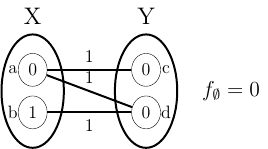
\includegraphics[scale=0.4]{img/toulbar2-0.png}
    \end{column}
\end{columns}
\begin{lstlisting}
solve ToWeighted(constraintPrefs1);
\end{lstlisting}
\begin{parchment}[Evaluationsfrage]
Wie schnell und effektiv (hinsichtlich des Findens von Optima) können Weighted-Instanzen durch klassische Constraint Solver gegenüber dedizierten Soft Constraint Solvern gelöst werden?
\end{parchment}
\end{frame}

\begin{frame}{Solver-Vergleich auf Weighted CSP I}
\vspace*{2ex}
\begin{table}
\centering
{
\scriptsize
\label{tab:resultsSolverComparison}

\begin{tabular*}{\textwidth}{@{\extracolsep{\fill} }ld{1.5}cd{1.5}d{1.1}d{1.1}}
\toprule
\multicolumn{1}{c}{Solver} & \multicolumn{1}{c}{Time (secs)} 
          & \multicolumn{1}{c}{\# Wins}
          & \multicolumn{1}{c}{Objective} 
          & \multicolumn{1}{c}{\% Solved} & \multicolumn{1}{c}{\% Optimal} \\
\midrule
\multicolumn{2}{l}{MSPSP (8 instances)  }   \\
\midrule
   Gecode & 0.32 \quad (1.00)& 8 & 2.50 \quad (0.00) & 100.00 & 100.00 \\
   G12 & 0.32 \quad (1.01)& 0 & 2.50 \quad (0.00) & 100.00 & 100.00 \\
   OR-Tools & 0.33 \quad (1.05)& 0 & 2.50 \quad (0.00) & 100.00 & 100.00 \\
   JaCoP & 0.52 \quad (1.73)& 0 & 2.50 \quad (0.00) & 100.00 & 100.00 \\
   Choco & 0.70 \quad (2.46)& 0 & 2.50 \quad (0.00) & 100.00 & 100.00 \\
   Toulbar2 & 312.56 \quad (1052.07)& 0 & 29.13 \quad (26.63) & 0.00 & 0.00 \\
\midrule
\multicolumn{2}{l}{On-Call Rostering (7 instances)  }   \\
\midrule
   Toulbar2 & 40.73 \quad (1.44)& 3 & 1.57 \quad (0.00) & 100.00 & 100.00 \\
   OR-Tools & 275.23 \quad (5.55)& 2 & 3.71 \quad (2.14) & 100.00 & 57.14 \\
   Gecode & 275.23 \quad (5.54)& 1 & 4.57 \quad (3.00) & 100.00 & 57.14 \\
   G12 & 276.36 \quad (5.63)& 1 & 5.57 \quad (4.00) & 100.00 & 57.14 \\
   JaCoP & 276.63 \quad (5.86)& 0 & 5.14 \quad (3.57) & 100.00 & 57.14 \\
   Choco & 276.72 \quad (6.26)& 0 & 5.14 \quad (3.57) & 100.00 & 57.14 \\
\midrule
\multicolumn{2}{l}{Photo Placement (3 instances)  }   \\
\midrule
   Toulbar2 & 0.80 \quad (1.11)& 0 & 13.33 \quad (0.00) & 100.00 & 100.00 \\
   Choco & 0.83 \quad (1.21)& 2 & 25.00 \quad (11.67) & 100.00 & 100.00 \\
   OR-Tools & 1.49 \quad (1.71)& 1 & 13.33 \quad (0.00) & 100.00 & 100.00 \\
   JaCoP & 3.18 \quad (3.61)& 0 & 13.33 \quad (0.00) & 100.00 & 100.00 \\
   Gecode & 22.24 \quad (21.62)& 0 & 13.33 \quad (0.00) & 100.00 & 100.00 \\
   G12 & 27.40 \quad (29.62)& 0 & 13.33 \quad (0.00) & 100.00 & 100.00 \\
\bottomrule
\end{tabular*}

}
\end{table}

\end{frame}

\begin{frame}{Solver-Vergleich auf Weighted CSP II}
\begin{table}
\centering
{
\scriptsize
\label{tab:resultsSolverComparison}

\begin{tabular*}{\textwidth}{@{\extracolsep{\fill} }ld{1.5}cd{1.5}d{1.1}d{1.1}}
\toprule
\multicolumn{1}{c}{Solver} & \multicolumn{1}{c}{Time (secs)} 
          & \multicolumn{1}{c}{\# Wins}
          & \multicolumn{1}{c}{Objective} 
          & \multicolumn{1}{c}{\% Solved} & \multicolumn{1}{c}{\% Optimal} \\
\midrule
\multicolumn{2}{l}{Soft N-Queens (3 instances)  }   \\
\midrule
   OR-Tools & 0.03 \quad (1.00)& 3 & 0.33 \quad (0.00) & 100.00 & 100.00 \\
   Toulbar2 & 0.30 \quad (10.43)& 0 & 0.33 \quad (0.00) & 100.00 & 100.00 \\
   Choco & 0.35 \quad (12.54)& 0 & 0.33 \quad (0.00) & 100.00 & 100.00 \\
   JaCoP & 57.22 \quad (1707.98)& 0 & 0.33 \quad (0.00) & 100.00 & 100.00 \\
   Gecode & 210.02 \quad (6266.00)& 0 & 1.67 \quad (1.33) & 100.00 & 66.67 \\
   G12 & 210.02 \quad (6266.14)& 0 & 1.67 \quad (1.33) & 100.00 & 66.67 \\
\midrule
\multicolumn{2}{l}{Talent Scheduling (7 instances)  }   \\
\midrule
   OR-Tools & 113.29 \quad (1.01)& 3 & 12.29 \quad (0.00) & 100.00 & 85.71 \\
   JaCoP & 117.71 \quad (1.84)& 0 & 12.29 \quad (0.00) & 100.00 & 85.71 \\
   Choco & 129.12 \quad (3.27)& 1 & 12.29 \quad (0.00) & 100.00 & 85.71 \\
   Toulbar2 & 158.27 \quad (60.70)& 0 & 28.43 \quad (16.14) & 28.57 & 28.57 \\
   Gecode & 183.29 \quad (4.70)& 3 & 12.29 \quad (0.00) & 100.00 & 85.71 \\
   G12 & 194.91 \quad (2.87)& 0 & 12.29 \quad (0.00) & 100.00 & 85.71 \\
\bottomrule
\end{tabular*}

}
\end{table}
\end{frame}

\begin{frame}[fragile]{Vergleich Constraint Preferences vs Weighted}
\vspace*{6ex}

\begin{columns}[onlytextwidth]
    \begin{column}{.45\textwidth}
    \centering \hFirst{Constraint Preferences}
    
    \vspace*{2ex}
    
\begin{tikzpicture}[auto,->,
                    >=stealth',shorten >=1pt,thick,
                    node distance=.7cm,inner sep=2pt,
                    constraint/.style={circle,fill=black!15,draw,font=\sffamily\small},
                    bg/.style={shape=rectangle, rounded corners,
    draw, align=center,
    top color=white, bottom color=issegrey!15},
                    pvs/.style={shape=rectangle, rounded corners,
    draw=isseorange!50,fill=white, align=center}]
 
\node[pvs,text width=4.8cm,anchor=north west, text height=2.8cm] at (5.7,-1) {};
\node at (9.4, -2.4) {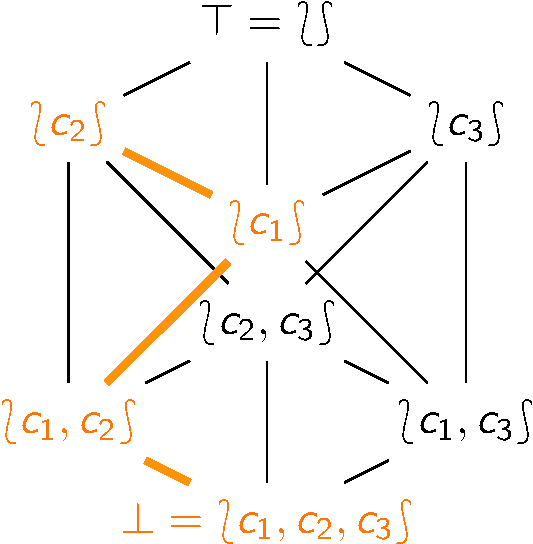
\includegraphics[width=2.3cm]{img/search-space.pdf} }; 

\node[anchor=west,font=\small] at (5.7,-1.3) {$\mathit{PVS}\langle P \rangle $};
\node[anchor=west,font=\normalsize] at (5.7,-3.6) {$\langle \finmsets(P), \mcup, \smytheq{P}, \lbag \rbag \rangle$};

\node[constraint,label=west:$\lbag \mathrm{c}_1 \rbag$] (p1) at (7, -2)                   {$\mathrm{c}_1$};
\node[constraint,label=east:$\lbag \mathrm{c}_2 \rbag$] (p2) at ($ (p1) + (-0.8, -0.8) $) {$\mathrm{c}_2$};  
\node[constraint,label=north:$\lbag \mathrm{c}_3 \rbag$] (p3) at ($ (p1) + ( 0.8, -0.8) $) {$\mathrm{c}_3$};  
%  
\path[every node/.style={font=\sffamily\tiny}]
  (p2) edge (p1)
  (p3) edge (p1)
  ;

\end{tikzpicture}

\begin{lstlisting}
solve constraintPrefs1;
\end{lstlisting}
    \end{column}
    \begin{column}{.45\textwidth}
    \centering \hSecond{Weighted}
    
    \vspace*{2ex}
    
    \begin{tikzpicture}[auto,->,
                    >=stealth',shorten >=1pt,thick,
                    node distance=.7cm,inner sep=2pt,
                    constraint/.style={circle,fill=black!15,draw,font=\sffamily\small},
                    bg/.style={shape=rectangle, rounded corners,
    draw, align=center,
    top color=white, bottom color=issegrey!15},
                    pvs/.style={shape=rectangle, rounded corners,
    draw=isseorange!50,fill=white, align=center}]

\node[pvs,draw=CornflowerBlue,text width=3.5cm,anchor=north west, text height=2.8cm] at (0.5,-1) {};
 \node[anchor=west,font=\small] at (0.5,-1.3) {$\mathit{Weighted}(P)$};
  \node[anchor=west,font=\normalsize] at (0.5,-3.6) {$\langle \mathbb{N}, +, \geq, 0 \rangle$};
  
\node[constraint,label=west:2] (w1) at (2, -2)                   {$\mathrm{c}_1$};
\node[constraint,label=west:1] (w2) at ($ (w1) + (-0.8, -0.8) $) {$\mathrm{c}_2$};  
\node[constraint,label=west:1] (w3) at ($ (w1) + ( 0.8, -0.8) $) {$\mathrm{c}_3$};  
\node at (3.6, -2.4) {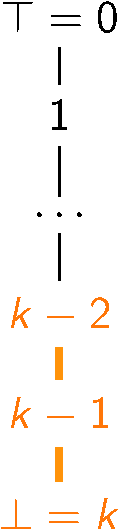
\includegraphics[width=.55cm]{img/search-space-weighted.pdf} }; 

%  
\path[every node/.style={font=\sffamily\tiny}]
  (w2) edge (w1)
  (w3) edge (w1)
  ;
 

\end{tikzpicture}
\begin{lstlisting}
solve ToWeighted(constraintPrefs1);
\end{lstlisting}
    \end{column}
  \end{columns}  
  
\begin{parchment}[Evaluationsfrage]
Ist es wesentlich teurer nach Smyth zu optimieren, anstatt ein gewichtetes Problem zu verwenden?

\end{parchment}
\end{frame}

\begin{frame}{Vergleich Weighted vs Constraint Preferences}
\vspace*{4ex}

\begin{table}
\centering
{
\scriptsize
\begin{tabular*}{\textwidth}{@{\extracolsep{\fill} }ld{1.1}d{1.1}d{1.1}d{1.1}d{1.1}}
\toprule
\multicolumn{1}{c}{Solver} & \multicolumn{1}{c}{Time Smyth} 
          & \multicolumn{1}{c}{Time Weighted} 
          & \multicolumn{1}{c}{Time Toulbar2}
          & \multicolumn{1}{c}{Obj. Weights} & \multicolumn{1}{c}{Obj. Smyth}   \\
\midrule
\multicolumn{2}{l}{MSPSP (6 instances)  }   \\
\midrule
   Gecode & 12.74 & \textbf{0}.\textbf{34} & - & 2.67 & 5.50 \\
   Native Gecode & 7.82 & \textbf{0}.\textbf{26} & - & 2.80 & 5.80 \\
   JaCoP & 4.18 & \textbf{0}.\textbf{45} & - & 2.00 & 6.00 \\
\midrule
\multicolumn{2}{l}{On-Call Rostering (5 instances)  }   \\
\midrule
   Gecode & 220.46 & \textbf{133}.\textbf{32} & (14.52) & 3.20 & 7.20 \\
   Native Gecode & 192.50 & \textbf{133}.\textbf{32} & (14.52) & 3.20 & 25.20 \\
   JaCoP & 194.06 & \textbf{135}.\textbf{28} & (14.52) & 3.20 & 26.80 \\
\midrule
\multicolumn{2}{l}{Photo Placement (3 instances)  }   \\
\midrule
   Gecode & 6.69 & \textbf{1}.\textbf{03} & (0.68) & 13.00 & 13.00 \\
   Native Gecode & \textbf{9}.\textbf{96} & 22.22 & (0.80) & 13.33 & 13.33 \\
   JaCoP & 15.73 & \textbf{3}.\textbf{18} & (0.80) & 13.33 & 13.33 \\
\midrule
\multicolumn{2}{l}{Soft N-Queens (3 instances)  }   \\
\midrule
   Gecode & \textbf{3}.\textbf{45} & 210.02 & (0.30) & 1.67 & 2.00 \\
   Native Gecode & \textbf{3}.\textbf{49} & 210.02 & (0.30) & 1.67 & 1.33 \\
   JaCoP & \textbf{3}.\textbf{94} & 57.22 & (0.30) & 0.33 & 1.00 \\
\midrule
\multicolumn{2}{l}{Talent Scheduling (6 instances)  }   \\
\midrule
   Gecode & \textbf{7}.\textbf{78} & 158.94 & - & 12.50 & 14.25 \\
   Native Gecode & \textbf{13}.\textbf{50} & 141.09 & - & 12.33 & 14.67 \\
   JaCoP & \textbf{15}.\textbf{63} & 120.42 & - & 12.33 & 14.17 \\
\bottomrule
\end{tabular*}

}
\end{table}
\end{frame}
\tikzstyle{highlight}=[isseorange,ultra thick]
\tikzstyle{highlight2}=[CornflowerBlue,ultra thick]

\begin{frame}[fragile]{Nicht-Dominiert versus Strikte Verbesserung}
\vspace*{6ex}

\begin{columns}[onlytextwidth]
    \begin{column}{.45\textwidth}
    \centering \hSecond{Nicht-Dominiert}
    
    \vspace*{2ex}
    
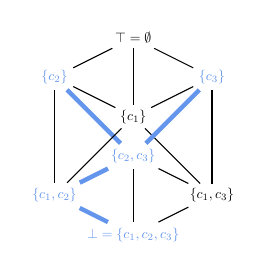
\begin{tikzpicture}[scale=0.5,transform shape,auto]

% single PVS
\node [highlight2] (bot) at (0,0) {$\bot = \{c_1, c_2, c_3 \}$};
\node [highlight2] (c1c2) at (-2,1) {$\{c_1, c_2\}$};
\node[highlight2] (c2c3) at (0,2) {$\{c_2, c_3\}$};
\node (c1c3) at (2,1) {$\{c_1, c_3\}$};

\node (c1) at (0,3) {$\{c_1\}$};
\node [highlight2] (c2) at (-2,4) {$\{c_2\}$};
\node [highlight2](c3) at (2,4) {$\{c_3\}$};
%\node (a) at (-1,0.5) {$a$};
%\node (b) at (-1,1.5) {$b$};
%\node (c) at (1,1) {$c$};
\node (top) at (0,5) {$\top = \emptyset$};


\path[-]
(bot) edge[highlight2](c1c2)
      edge (c2c3)
      edge (c1c3)
(c1c2) edge[highlight2] (c2c3)
(c1c3) edge (c2c3)
(c1c3) edge (c1)
(c1c3) edge (c3)
(c2c3) edge[highlight2] (c2)
(c2c3) edge[highlight2] (c3)
(c1c2) edge (c1)
(c1c2) edge (c2)
(c1) edge (c2)
(c1) edge (c3)
(c2) edge (top)
(c1) edge (top)
(c3) edge (top)
      ;

\end{tikzpicture}

\begin{lstlisting}
solve 
search pvs_BAB_NonDom();  
\end{lstlisting}
    \end{column}
    \begin{column}{.45\textwidth}
    \centering \hFirst{Strikte Verbesserung}
    
    \vspace*{2ex}
    
\begin{tikzpicture}[scale=0.5,transform shape,auto]

% single PVS
\node (bot) at (0,0) {\alert{$\bot = \{c_1, c_2, c_3 \}$}};
\node (c1c2) at (-2,1) {\alert{$\{c_1, c_2\}$}};
\node (c2c3) at (0,2) {\alert{$\{c_2, c_3\}$}};
\node (c1c3) at (2,1) {$\{c_1, c_3\}$};

\node (c1) at (0,3) {$\{c_1\}$};
\node (c2) at (-2,4) {\alert{$\{c_2\}$}};
\node (c3) at (2,4) {$\{c_3\}$};
%\node (a) at (-1,0.5) {$a$};
%\node (b) at (-1,1.5) {$b$};
%\node (c) at (1,1) {$c$};
\node (top) at (0,5) {$\top = \emptyset$};


\path[-]
(bot) edge[highlight] (c1c2)
      edge (c2c3)
      edge (c1c3)
(c1c2) edge[highlight]  (c2c3)
(c1c3) edge (c2c3)
(c1c3) edge (c1)
(c1c3) edge (c3)
(c2c3) edge[highlight]  (c2)
(c2c3) edge (c3)
(c1c2) edge (c1)
(c1c2) edge (c2)
(c1) edge (c2)
(c1) edge (c3)
(c2) edge (top)
(c1) edge (top)
(c3) edge (top)
      ;

\end{tikzpicture}

\begin{lstlisting}
solve 
search pvs_BAB();  
\end{lstlisting}
    \end{column}
  \end{columns}  
  
\begin{parchment}[Evaluationsfrage]
Wieviel Overhead erzeugt das Suchen aller (unvergleichbar) optimalen Lösungen gegenüber dem Suchein \emph{einer} optimalen Lösung?
\end{parchment}
\end{frame}


\begin{frame}[fragile]{Nicht-Dominiert versus Strikte Verbesserung}
\begin{columns}[onlytextwidth]
    \begin{column}{.45\textwidth}
    \centering \hSecond{Nicht-Dominiert}
    
    \vspace*{2ex}
    
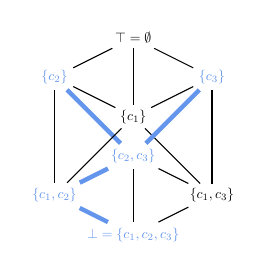
\begin{tikzpicture}[scale=0.5,transform shape,auto]

% single PVS
\node [highlight2] (bot) at (0,0) {$\bot = \{c_1, c_2, c_3 \}$};
\node [highlight2] (c1c2) at (-2,1) {$\{c_1, c_2\}$};
\node[highlight2] (c2c3) at (0,2) {$\{c_2, c_3\}$};
\node (c1c3) at (2,1) {$\{c_1, c_3\}$};

\node (c1) at (0,3) {$\{c_1\}$};
\node [highlight2] (c2) at (-2,4) {$\{c_2\}$};
\node [highlight2](c3) at (2,4) {$\{c_3\}$};
%\node (a) at (-1,0.5) {$a$};
%\node (b) at (-1,1.5) {$b$};
%\node (c) at (1,1) {$c$};
\node (top) at (0,5) {$\top = \emptyset$};


\path[-]
(bot) edge[highlight2](c1c2)
      edge (c2c3)
      edge (c1c3)
(c1c2) edge[highlight2] (c2c3)
(c1c3) edge (c2c3)
(c1c3) edge (c1)
(c1c3) edge (c3)
(c2c3) edge[highlight2] (c2)
(c2c3) edge[highlight2] (c3)
(c1c2) edge (c1)
(c1c2) edge (c2)
(c1) edge (c2)
(c1) edge (c3)
(c2) edge (top)
(c1) edge (top)
(c3) edge (top)
      ;

\end{tikzpicture}

    \end{column}
    \begin{column}{.45\textwidth}
    \centering \hFirst{Strikte Verbesserung}
    
    \vspace*{2ex}
    
\begin{tikzpicture}[scale=0.5,transform shape,auto]

% single PVS
\node (bot) at (0,0) {\alert{$\bot = \{c_1, c_2, c_3 \}$}};
\node (c1c2) at (-2,1) {\alert{$\{c_1, c_2\}$}};
\node (c2c3) at (0,2) {\alert{$\{c_2, c_3\}$}};
\node (c1c3) at (2,1) {$\{c_1, c_3\}$};

\node (c1) at (0,3) {$\{c_1\}$};
\node (c2) at (-2,4) {\alert{$\{c_2\}$}};
\node (c3) at (2,4) {$\{c_3\}$};
%\node (a) at (-1,0.5) {$a$};
%\node (b) at (-1,1.5) {$b$};
%\node (c) at (1,1) {$c$};
\node (top) at (0,5) {$\top = \emptyset$};


\path[-]
(bot) edge[highlight] (c1c2)
      edge (c2c3)
      edge (c1c3)
(c1c2) edge[highlight]  (c2c3)
(c1c3) edge (c2c3)
(c1c3) edge (c1)
(c1c3) edge (c3)
(c2c3) edge[highlight]  (c2)
(c2c3) edge (c3)
(c1c2) edge (c1)
(c1c2) edge (c2)
(c1) edge (c2)
(c1) edge (c3)
(c2) edge (top)
(c1) edge (top)
(c3) edge (top)
      ;

\end{tikzpicture}

    \end{column}
  \end{columns}  
\begin{table}
\centering
{
\scriptsize

\label{tab:compDomNonDom}


\begin{tabular*}{\textwidth}{@{\extracolsep{\fill} }ld{1.1}d{1.1}d{1.1}d{1.1}}
\toprule
\multicolumn{1}{c}{Problem} & \multicolumn{1}{c}{Time Non-Dominated BaB} 
          & \multicolumn{1}{c}{Time Strict BaB} 
          & \multicolumn{1}{c}{Absolute Overhead}
          & \multicolumn{1}{c}{Relative Overhead}   \\
\midrule
   MSPSP & \textbf{7}.\textbf{31} & 8.89 & -1.58 & 1.50 \\
   On-Call Rostering & 329.44 & \textbf{199}.\textbf{21} & 130.23 & 1.82 \\
   Photo Placement & 55.09 & \textbf{7}.\textbf{51} & 47.58 & 9.72 \\
   Soft N-Queens & \textbf{2}.\textbf{24} & 3.65 & -1.41 & 1.91 \\
   Talent Scheduling & 33.44 & \textbf{12}.\textbf{24} & 21.21 & 2.30 \\
\midrule
\emph{Overall} & 102.00 & \textbf{57}.\textbf{20} & 44.80 & 2.97 \\
\bottomrule
\end{tabular*}
}
\end{table}

\end{frame}

\begin{frame}[fragile]{Vergleich MIF vs. Standard}
\vspace*{2ex}

\begin{lstlisting}
type WeightedCsp = PVSType<bool, int> = 
  params {[..]  } in  
  instantiates with "soft_constraints/mbr_types/weighted_type.mzn" { [...] }
 offers {
    heuristics -> getSearchHeuristicWeighted;
 };
 \end{lstlisting}

\begin{columns}[onlytextwidth]
    \begin{column}{.45\textwidth}
    \centering \hFirst{Most-Important First}

    \vspace*{1ex}

\begin{lstlisting}
solve 
:: pvsSearchHeuristic
search pvs_BAB();
\end{lstlisting}
    \end{column}
    \begin{column}{.45\textwidth}
    \centering \hSecond{Standard-Suche}

    \vspace*{1ex}
    \begin{lstlisting}
solve 
search pvs_BAB();
\end{lstlisting}
    \end{column}
\end{columns}
\begin{parchment}[Evaluationsfrage]
Kann die generische MIF-Suchheuristik die Suche nach Optima beschleunigen?
\end{parchment}
\end{frame}

\begin{frame}{Vergleich MIF vs. Standard I}
\begin{table}
\centering
{
\scriptsize

\label{tab:compDiffsMif}


\subcaption*{Gruppiert nach Solvern.}
\begin{tabular*}{\textwidth}{@{\extracolsep{\fill} }ld{1.1}d{1.1}d{1.1}d{1.1}d{1.1}d{1.1}d{1.1}}
\toprule
 &  \multicolumn{1}{c}{Choco} & \multicolumn{1}{c}{G12} & \multicolumn{1}{c}{Gecode} & \multicolumn{1}{c}{JaCoP} & \multicolumn{1}{c}{Toulbar2} & \multicolumn{1}{c}{OR-Tools} \\
\midrule
Instances &  28 & 28 & 28 & 28 & 28 & 28 \\
Runtime difference &  -73.14 & -17.57 & -18.42 & 16.15 & 36.63 & 19.05 \\
Ratio MIF wins &  0.64 & 0.32 & 0.29 & 0.46 & 0.57 & 0.32 \\
\bottomrule
\end{tabular*}

\bigskip
\subcaption*{Gruppiert nach Problemen.}

\begin{tabular*}{\textwidth}{@{\extracolsep{\fill} }ld{1.1}d{1.1}d{1.1}d{1.1}d{1.1}d{1.1}}
\toprule
 &  \multicolumn{1}{c}{MSPSP} & \multicolumn{1}{c}{On-Call Rostering} & \multicolumn{1}{c}{Photo Placement} & \multicolumn{1}{c}{Soft N-Queens} & \multicolumn{1}{c}{Talent Scheduling} \\
\midrule
Instances &  48 & 42 & 18 & 18 & 42 \\
Runtime difference &  -0.80 & -31.04 & 141.17 & -79.51 & -19.34 \\
Ratio MIF wins &  0.42 & 0.55 & 0.06 & 0.56 & 0.45 \\
\bottomrule
\end{tabular*}
}
\end{table}
\end{frame}

\begin{frame}{Vergleich MIF vs. Standard II}
\begin{figure}
	\centering
	\begin{subfigure}[b]{.48\textwidth}
		\centering
		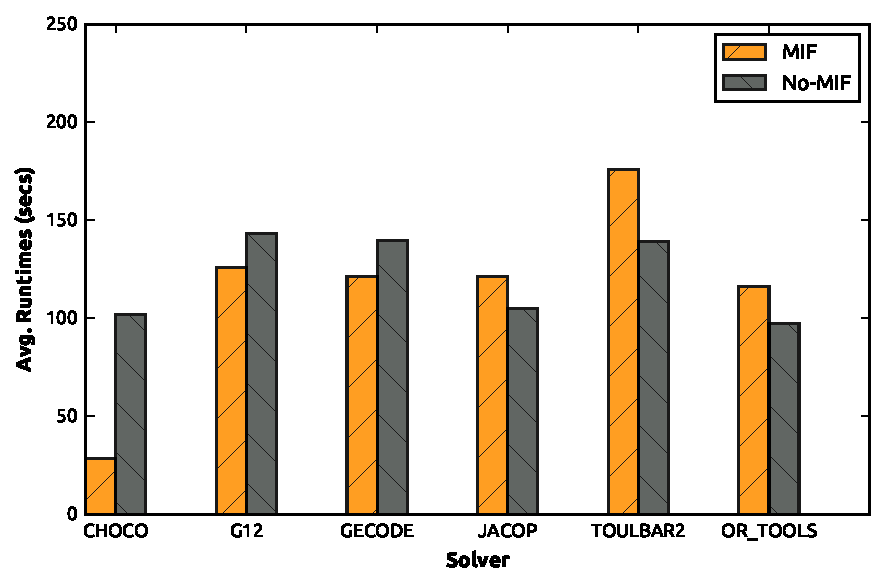
\includegraphics[width=\textwidth]{img/runtime-mif-solver.pdf} %TODO: check: how were the 8 points sampled? Not uniformly...
         \caption{Runtimes grouped by solver for MIF on/off.}
		\label{fig:runtimesMIFSolvers}
	\end{subfigure}%
	~ \quad%add desired spacing between images, e. g. ~, \quad, \qquad, \hfill etc.
	%(or a blank line to force the subfigure onto a new line)
	\begin{subfigure}[b]{.48\textwidth}
		\centering
		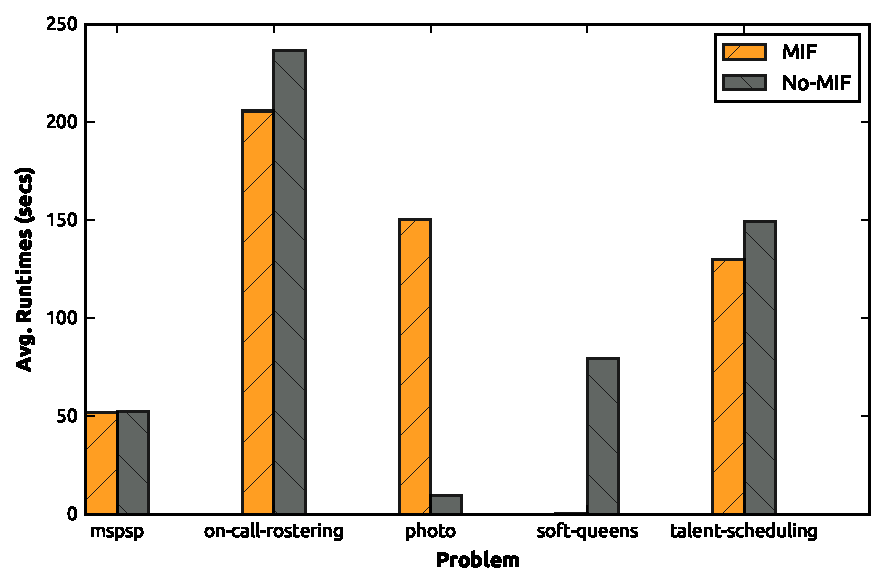
\includegraphics[width=\textwidth]{img/runtime-mif-problem.pdf}
		\caption{Runtimes grouped by problem for MIF on/off.}
		\label{fig:runtimesMIFProblems}
	\end{subfigure}

	\label{fig:runtimesMIF}
\end{figure}
\end{frame}